% -----------------------------*- LaTeX -*------------------------------
\documentclass[UTF8]{report}
% ------------------------------------------------------------------------
% Packages
% ------------------------------------------------------------------------
\usepackage{ctex} % 支持中文
\usepackage[body={7in, 9in},left=1in,right=1in]{geometry} % 改变页边距
\usepackage{amsmath} % AMS 的数学宏包
\usepackage{amsfonts} % AMS 的数学字体宏包
\usepackage{amssymb} % AMS 符号库
\usepackage{bm} % 数学公式中的黑斜体
\usepackage{amsthm} % AMS 的定理环境宏包
\usepackage{graphicx} % 插图
\usepackage{subfigure} % 插子图
\usepackage{nicefrac} % 好看的分数
\usepackage{mathrsfs} % mathscr font
\usepackage{caption} % caption
\usepackage{algorithm,algorithmicx} % 伪代码支持宏包
\usepackage[noend]{algpseudocode} % 伪代码
\usepackage{fancyhdr} % 设置页眉、页脚
\usepackage{adjustbox} % 图片尺寸自动调整
\usepackage{esint} % 积分符号
\usepackage{mathtools} % 数学宏包的重要补充
\usepackage{upgreek} % 数学环境的直立希腊字母
\usepackage{enumitem} % 使用enumitem宏包, 改变列表项的格式
\usepackage{color} % 支持彩色
\usepackage{extarrows} % 任意长度的箭头
\usepackage{tikz} % 绘图
\usepackage{forest} % 绘树
\usepackage{xcolor} % 颜色宏包
\usepackage{breqn} % 公式自动换行
\usepackage{fontsize} % 字体大小
\usepackage[framemethod=TikZ]{mdframed} % 给文字加框
\usepackage{fontspec} % 字体库
\usepackage{bigstrut} % 用于表格中的换行
\usepackage{multirow} % 表格中多行单元格合并
\usepackage{multicol} % 表格中多列单元格合并
\usepackage{longtable} % 长表格
\usepackage{rotating} % 旋转图形和表格      以上三者用于绘制三线表
\usepackage{booktabs} % 三线表宏包
\usepackage{scribe} % Scribe 模板
\usepackage{diagbox} % 表格斜线
\usepackage{listings} % 插入代码
\usepackage{verbatim} % 多行注释
\usetikzlibrary{shapes.geometric, arrows} % 引入流程图需要的库
\usetikzlibrary{automata} % 引入automata库
\usetikzlibrary{shapes,arrows,positioning,chains} % 引入positioning库
% ------------------------------------------------------------------------
% Macros
% ------------------------------------------------------------------------
%~~~~~~~~~~~~~~~
% Utility latin
%~~~~~~~~~~~~~~~
\newcommand{\ie}{\textit{i.e.}}
\newcommand{\eg}{\textit{e.g.}}
%~~~~~~~~~~~~~~~
% Environment shortcuts
%~~~~~~~~~~~~~~~
\newcommand{\balign}[1]{\ealign{\begin{align}#1\end{align}}}
\newcommand{\baligns}[1]{\ealigns{\begin{align*}#1\end{align*}}}
\newcommand{\bitemize}[1]{\eitemize{\begin{itemize}#1\end{itemize}}}
\newcommand{\benumerate}[1]{\eenumerate{\begin{enumerate}#1\end{enumerate}}}
%~~~~~~~~~~~~~~~
% Text with quads around it
%~~~~~~~~~~~~~~~
\newcommand{\qtext}[1]{\quad\text{#1}\quad}
%~~~~~~~~~~~~~~~
% Shorthand for math formatting
%~~~~~~~~~~~~~~~
\newcommand{\mbb}[1]{\mathbb{#1}}
\newcommand{\mbi}[1]{\boldsymbol{#1}} % Bold and italic (math bold italic)
\newcommand{\mbf}[1]{\mathbf{#1}}
\newcommand{\mc}[1]{\mathcal{#1}}
\newcommand{\mrm}[1]{\mathrm{#1}}
\newcommand{\tbf}[1]{\textbf{#1}}
\newcommand{\tsc}[1]{\textsc{#1}}
%\def\\langle {{\langle }}
%\def\\rangle {{\rangle }}
\newcommand{\sT}{\sf T}
\newcommand{\grad}{\nabla}
\newcommand{\Proj}{\Pi}
%~~~~~~~~~~~~~~~
% Common sets 定义数集符号
%~~~~~~~~~~~~~~~
\newcommand{\R}{\mathbb{R}}
\newcommand{\Z}{\mathbb{Z}}
\newcommand{\Q}{\mathbb{Q}}
\newcommand{\N}{\mathbb{N}}
\newcommand{\C}{\mathbb{C}}
\newcommand{\reals}{\mathbb{R}} % Real number symbol
\newcommand{\integers}{\mathbb{Z}} % Integer symbol
\newcommand{\rationals}{\mathbb{Q}} % Rational numbers
\newcommand{\naturals}{\mathbb{N}} % Natural numbers
\newcommand{\complex}{\mathbb{C}} % Complex numbers
%~~~~~~~~~~~~~~~
% Common functions
%~~~~~~~~~~~~~~~
\renewcommand{\exp}[1]{\operatorname{exp}\left(#1\right)} % Exponential
\newcommand{\indic}[1]{\mbb{I}\left(#1\right)} % Indicator function
\newcommand{\indicsub}[2]{\mbb{I}_{#2}\left(#1\right)} % Indicator function
\newcommand{\argmax}{\mathop\mathrm{arg\, max}} % Defining math symbols
\newcommand{\argmin}{\mathop\mathrm{arg\, min}}
\renewcommand{\arccos}{\mathop\mathrm{arccos}}
\newcommand{\dom}{\mathop\mathrm{dom}} % Domain
\newcommand{\range}{\mathop\mathrm{range}} % Range
\newcommand{\diag}{\mathop\mathrm{diag}}
\newcommand{\tr}{\mathop\mathrm{tr}}
\newcommand{\abs}{\mathop\mathrm{abs}}
\newcommand{\card}{\mathop\mathrm{card}}
\newcommand{\sign}{\mathop\mathrm{sign}}
\newcommand{\prox}{\mathrm{prox}} % prox
\newcommand{\rank}[1]{\mathrm{rank}(#1)}
\newcommand{\supp}[1]{\mathrm{supp}(#1)}
\newcommand{\norm}[1]{\lVert#1\rVert}
%~~~~~~~~~~~~~~~
% Common probability symbols
%~~~~~~~~~~~~~~~
\newcommand{\family}{\mathcal{P}} % probability family / statistical model
\newcommand{\iid}{\stackrel{\mathrm{iid}}{\sim}}
\newcommand{\ind}{\stackrel{\mathrm{ind}}{\sim}}
\newcommand{\E}{\mathbb{E}} % Expectation symbol
\newcommand{\Earg}[1]{\E\left[#1\right]}
\newcommand{\Esubarg}[2]{\E_{#1}\left[#2\right]}
\renewcommand{\P}{\mathbb{P}} % Probability symbol
\newcommand{\Parg}[1]{\P\left(#1\right)}
\newcommand{\Psubarg}[2]{\P_{#1}\left[#2\right]}
%\newcommand{\Cov}{\mrm{Cov}} % Covariance symbol
%\newcommand{\Covarg}[1]{\Cov\left[#1\right]}
%\newcommand{\Covsubarg}[2]{\Cov_{#1}\left[#2\right]}
%\newcommand{\model}{\mathcal{P}} % probability family / statistical model
%~~~~~~~~~~~~~~~
% Distributions
%~~~~~~~~~~~~~~~
%\newcommand{\Gsn}{\mathcal{N}}
%\newcommand{\Ber}{\textnormal{Ber}}
%\newcommand{\Bin}{\textnormal{Bin}}
%\newcommand{\Unif}{\textnormal{Unif}}
%\newcommand{\Mult}{\textnormal{Mult}}
%\newcommand{\NegMult}{\textnormal{NegMult}}
%\newcommand{\Dir}{\textnormal{Dir}}
%\newcommand{\Bet}{\textnormal{Beta}}
%\newcommand{\Gam}{\textnormal{Gamma}}
%\newcommand{\Poi}{\textnormal{Poi}}
%\newcommand{\HypGeo}{\textnormal{HypGeo}}
%\newcommand{\GEM}{\textnormal{GEM}}
%\newcommand{\BP}{\textnormal{BP}}
%\newcommand{\DP}{\textnormal{DP}}
%\newcommand{\BeP}{\textnormal{BeP}}
%\newcommand{\Exp}{\textnormal{Exp}}
%~~~~~~~~~~~~~~~
% Theorem-like environments
%~~~~~~~~~~~~~~~
%\theoremstyle{definition}
%\newtheorem{definition}{Definition}
%\newtheorem{example}{Example}
%\newtheorem{problem}{Problem}
%\newtheorem{lemma}{Lemma}
%~~~~~~~~~~~~~~~
% 组合数学的模板和作业里用到的一些宏包和自定义命令
%~~~~~~~~~~~~~~~
\renewcommand{\emph}[1]{\begin{kaishu}#1\end{kaishu}}
\newcommand{\falfac}[1]{^{\underline{#1}}}
\newcommand{\binomfrac}[2]{\frac{#1^{\underline{#2}}}{#2!}}
\newcommand{\ceil}[1]{\left\lceil #1 \right\rceil}
\newcommand{\floor}[1]{\left\lfloor #1 \right\rfloor}
\newcommand{\suminfty}[2]{\sum_{#1=#2}^{\infty}}
\newcommand{\suminftyk}[0]{\sum_{k=0}^{\infty}}
\newcommand{\sumint}[3]{\sum_{#1=#2}^{#3}}
\newcommand{\sumintk}[2]{\sum_{k=#1}^{#2}}
\newcommand{\suminti}[2]{\sum_{i=#1}^{#2}}
%~~~~~~~~~~~~~~~
% 定义新命令
%~~~~~~~~~~~~~~~
\newcommand*{\unit}[1]{\mathop{}\!\mathrm{#1}}
\newcommand*{\dif}{\mathop{}\!\mathrm{d}}%微分算子 d
\newcommand*{\pdif}{\mathop{}\!\partial}%偏微分算子
\newcommand*{\cdif}{\mathop{}\!\nabla}%协变导数、nabla 算子
\newcommand*{\laplace}{\mathop{}\!\Delta}%laplace 算子
\newcommand*{\deri}[1]{\mathrm{d} #1}
\newcommand*{\deriv}[2]{\frac{\mathrm{d} #1}{\mathrm{d} {#2}}}
\newcommand*{\derivh}[3]{\frac{\mathrm{d}^{#1} #2}{\mathrm{d} {#3^{#1}}}}
\newcommand*{\pderiv}[2]{\frac{\partial #1}{\partial {#2}}}
\newcommand*{\pderivh}[3]{\frac{\partial^{#1} #2}{\partial {#3^{#1}}}}
\newcommand*{\dderiv}[2]{\dfrac{\mathrm{d} #1}{\mathrm{d} {#2}}}
\newcommand*{\dderivh}[3]{\dfrac{\mathrm{d}^{#1} #2}{\mathrm{d} {#3^{#1}}}}
\newcommand*{\dpderiv}[2]{\dfrac{\partial #1}{\partial {#2}}}
\newcommand*{\dpderivh}[3]{\dfrac{\partial^{#1} #2}{\partial {#3^{#1}}}}
\newcommand{\me}[1]{\mathrm{e}^{#1}}%e 指数
\newcommand{\mi}{\mathrm{i}}%虚数单位
%\newcommand{\mc}{\mathrm{c}}%光速 定义与mathcal冲突
\newcommand{\red}[1]{\textcolor{red}{#1}}
\newcommand{\blue}[1]{\textcolor{blue}{#1}}
%\newcommand{\Rome}[1]{\setcounter{rome}{#1}\Roman{rome}}
%~~~~~~~~~~~~~~~
% 公式环境中箭头符号的简写
%~~~~~~~~~~~~~~~
\newcommand{\ra}{\rightarrow}
\newcommand{\Ra}{\Rightarrow}
\newcommand{\la}{\leftarrow}
\newcommand{\La}{\Leftarrow}
\newcommand{\lra}{\leftrightarrow}
\newcommand{\Lra}{\Leftrightarrow}
\newcommand{\lgla}{\longleftarrow}
\newcommand{\Lgla}{\Longleftarrow}
\newcommand{\lgra}{\longrightarrow}
\newcommand{\Lgra}{\Longrightarrow}
\newcommand{\lglra}{\longleftrightarrow}
\newcommand{\Lglra}{\Longleftrightarrow}
%~~~~~~~~~~~~~~~
% 一些数学的环境设置
%~~~~~~~~~~~~~~~
%\newcounter{counter_exm}\setcounter{counter_exm}{1}
%\newcounter{counter_prb}\setcounter{counter_prb}{1}
%\newcounter{counter_thm}\setcounter{counter_thm}{1}
%\newcounter{counter_lma}\setcounter{counter_lma}{1}
%\newcounter{counter_dft}\setcounter{counter_dft}{1}
%\newcounter{counter_clm}\setcounter{counter_clm}{1}
%\newcounter{counter_cly}\setcounter{counter_cly}{1}
\newtheorem{theorem}{{\hskip 1.7em \bf 定理}}
\newtheorem{lemma}[theorem]{\hskip 1.7em 引理}
\newtheorem{proposition}[theorem]{\hskip 1.7em 命题}
\newtheorem{claim}[theorem]{\hskip 1.7em 断言}
\newtheorem{corollary}[theorem]{\hskip 1.7em 推论}
% \newcommand{\problem}[1]{{\setlength{\parskip}{10pt}\noindent \bf{#1}}}
\newenvironment{solution}{{\noindent \bf 解 \quad}}{}
\newenvironment{remark}{{\noindent \bf 注 \quad}}{}
\newenvironment{definition}{{\noindent \bf 定义 \quad}}{}
\renewenvironment{proof}{{\setlength{\parskip}{7pt}\noindent\hskip 2em \bf 证明 \quad}}{\hfill$\qed$\par}
\newenvironment{example}{{\noindent\bf 例 \quad}}{\hfill$\qed$\par}
%\newenvironment{concept}[1]{{\bf #1\quad} \begin{kaishu}} {\end{kaishu}\par}
%~~~~~~~~~~~~~~~
% 本.tex文档中特殊定义命令
%~~~~~~~~~~~~~~~
\newcommand{\lno}[1]{\overline{#1}}
\newcommand{\NP}{\mathrm{NP}}
\newcommand{\coNP}{\mathrm{coNP}}
% \newcommand{\ISO}{\mathrm{ISO}}
\newcommand{\SAT}{\mathrm{SAT}}
\newcommand{\USAT}{\mathrm{USAT}}
% \newcommand{\threeSAT}{\mathrm{3\text{-}SAT}}
\renewcommand{\P}{\mathrm{P}}
% \mathchardef\mhyphen="2D
% \newcommand{\CNF}{\mathrm{CNF}}
% \newcommand{\DNF}{\mathrm{DNF}}
% \newcommand{\SetSp}{\mathrm{SET\text{-}SPLITTING}}
% \newcommand{\PUZZLE}{\mathrm{PUZZLE}}
% \newcommand{\SPATH}{\mathrm{SPATH}}
% \newcommand{\LPATH}{\mathrm{LPATH}}
% \newcommand{\UHAMPATH}{\mathrm{UHAMPATH}}
\newcommand{\SPACE}{\mathrm{SPACE}}
\newcommand{\NSPACE}{\mathrm{NSPACE}}
\newcommand{\PSPACE}{\mathrm{PSPACE}}
\newcommand{\NPSPACE}{\mathrm{NPSPACE}}
\newcommand{\DFA}{\mathrm{DFA}}
\newcommand{\NFA}{\mathrm{NFA}}
\newcommand{\TQBF}{\mathrm{TQBF}}
% \newcommand{\L}{\mathrm{L}}
\renewcommand{\O}{\mathrm{O}}
\newcommand{\NL}{\mathrm{NL}}
\newcommand{\coNL}{\mathrm{coNL}}
\newcommand{\LADDER}{\mathrm{LADDER_{DFA}}}
\newcommand{\hd}{\mathrm{\text{-}hard}}
\newcommand{\ADD}{\mathrm{ADD}}
\newcommand{\STCN}{\mathrm{STRONGLY\text{-}CONNECTED}}
\newcommand{\PATH}{\mathrm{PATH}}
\newcommand{\A}{\mathrm{A}}
%使用align环境公式换页
\allowdisplaybreaks[4]

\definecolor{dkgreen}{rgb}{0,0.6,0}
\definecolor{gray}{rgb}{0.5,0.5,0.5}
\definecolor{mauve}{rgb}{0.58,0,0.82}
\lstset{
  frame=tb,
  aboveskip=3mm,
  belowskip=3mm,
  showstringspaces=false,
  columns=flexible,
  framerule=1pt,
  rulecolor=\color{gray!35},
  backgroundcolor=\color{gray!5},
  basicstyle={\small\ttfamily},
  numbers=none,
  numberstyle=\tiny\color{gray},
  keywordstyle=\color{blue},
  commentstyle=\color{dkgreen},
  stringstyle=\color{mauve},
  breaklines=true,
  breakatwhitespace=true,
  tabsize=3,
}

\tikzstyle{startstop} = [rectangle, rounded corners, minimum width=3cm, minimum height=1cm,text centered, draw=black, fill=red!30]
\tikzstyle{process} = [rectangle, minimum width=3cm, minimum height=1cm, text centered, draw=black, fill=orange!30]
\tikzstyle{decision} = [diamond, minimum width=3cm, minimum height=1cm, text centered, draw=black, fill=green!30]
\tikzstyle{arrow} = [thick,->,>=stealth]

\setmainfont{Times New Roman}
\setsansfont{Times New Roman}
\setmonofont{Consolas}
\setCJKmainfont{SimHei}
\setCJKsansfont{SimSun}
\setCJKmonofont{FangSong}
\punctstyle{kaiming}

\begin{document}

\pagestyle{fancy}

\reporttype{Report}                 % required
\course{Lab of Computer Architecture} 				% optional
\coursetitle{Pipeline}	    % optional
\semester{Fall 2024}			    % optional
\lecturer{Wang Wenxiang}			% optional
\scribe{Zhang Jiawei}			% required
\lecturenumber{2}				% required (must be a number)
\lecturedate{September 20}			% required (omit year)
\maketitle

\section{实验任务}

\begin{enumerate}
    \item exp7: 通过修改单周期CPU代码,实现一个不考虑数据冲突的简单流水线处理器,包括取指、译码、执行、访存和写回五个阶段。
    \item exp8: 在流水线处理器的基础上,实现冲突时阻塞流水级,解决数据冲突。
    \item exp9: 在流水线处理器的基础上,实现冲突时进行数据前递,解决数据冲突,提高流水线效率。
\end{enumerate}

\section{实验设计}

下面给出大致设计框图:
\begin{center}
    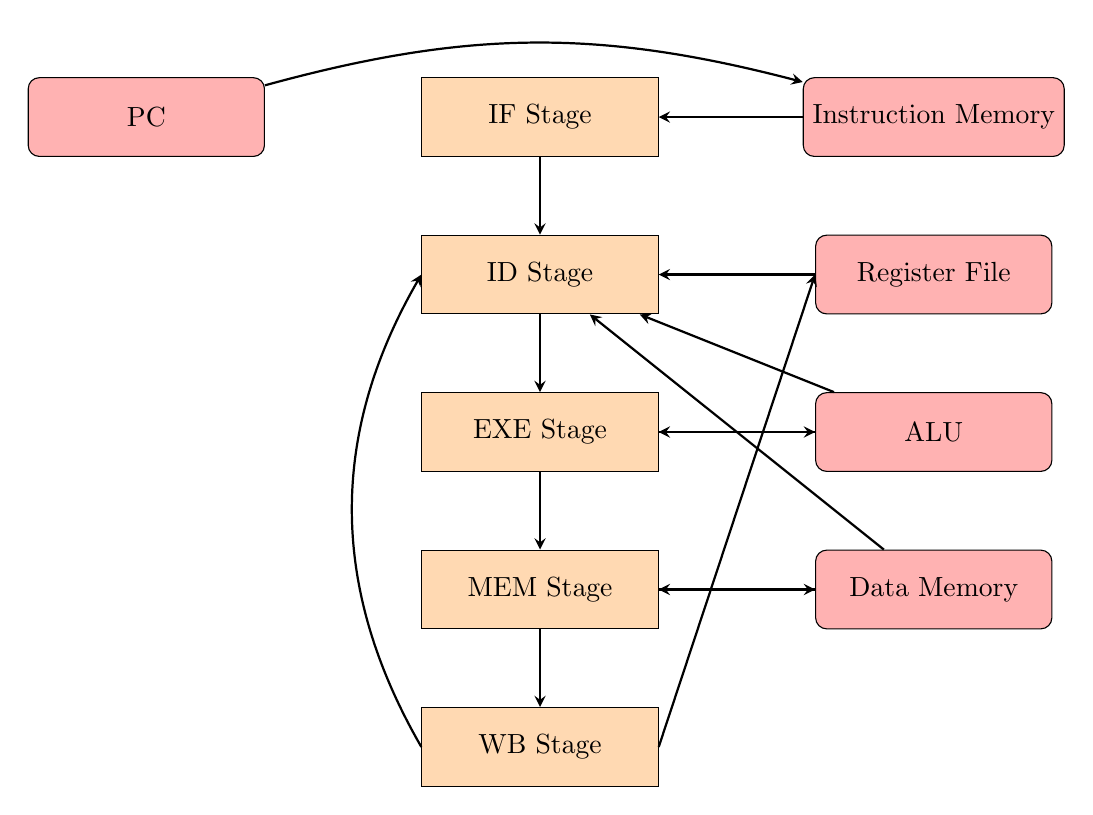
\begin{tikzpicture}[node distance=2cm]
        % Nodes for pipeline stages
        \node (if_stage) [process] {IF Stage};
        \node (id_stage) [process, below of=if_stage] {ID Stage};
        \node (exe_stage) [process, below of=id_stage] {EXE Stage};
        \node (mem_stage) [process, below of=exe_stage] {MEM Stage};
        \node (wb_stage) [process, below of=mem_stage] {WB Stage};
        
        % Connections between pipeline stages
        \draw [arrow] (if_stage) -- (id_stage);
        \draw [arrow] (id_stage) -- (exe_stage);
        \draw [arrow] (exe_stage) -- (mem_stage);
        \draw [arrow] (mem_stage) -- (wb_stage);
        
        % Instruction Fetch (IF) Stage Signals
        \node (pc) [startstop, left of=if_stage, xshift=-3cm] {PC};
        
        \node (inst_mem) [startstop, right of=if_stage, xshift=3cm] {Instruction Memory};
        \draw [arrow] (inst_mem) -- (if_stage);
        \draw [arrow, bend left=15] (pc) to (inst_mem);
        
        % Instruction Decode (ID) Stage Signals
        \node (reg_file) [startstop, right of=id_stage, xshift=3cm] {Register File};
        \draw [arrow] (reg_file) -- (id_stage);
        
        % Execute (EXE) Stage Signals
        \node (alu) [startstop, right of=exe_stage, xshift=3cm] {ALU};
        \draw [arrow] (exe_stage) -- (alu);
        \draw [arrow] (alu) --  (id_stage);
        \draw [arrow] (alu) --  (exe_stage);
        
        % Memory Access (MEM) Stage Signals
        \node (data_mem) [startstop, right of=mem_stage, xshift=3cm] {Data Memory};
        \draw [arrow] (mem_stage) -- (data_mem);
        \draw [arrow] (data_mem) -- (mem_stage);
        \draw [arrow] (data_mem) -- (id_stage);
        
        % Write Back (WB) Stage Signals
        \draw [arrow] (wb_stage.east) to (reg_file.west);
        \draw [arrow, bend left] (wb_stage.west) to (id_stage.west);
    \end{tikzpicture}
\end{center}

IF阶段从指令存储器中读取指令,ID阶段进行译码,获取各个控制信号,并从寄存器堆中读取数据(可能是前递的数据),EXE阶段进行运算,MEM阶段访问数据存储器,WB阶段将结果写回寄存器堆,这便是设计思路。当然,具体实现要比这个复杂得多,需要考虑各种情况。数据怎么在流水级之间传递?怎么判定数据冲突?数据冲突的时候应该怎么办?分支指令怎么处理?应该怎样用控制信号来控制流水线的暂停和恢复?这些问题就是实验过程中我们需要解决的问题,也是这三次实验的重点。

\subsection{流水线所使用的控制信号}

我们的流水线总共有五个阶段,每个阶段都需要各自的控制信号。valid指示当前阶段是否有效,allowin指示是否允许该个阶段接收数据,readygo指示是否允许该阶段向下一个阶段传递数据,pass指示数据是否能够通过该阶段。以EXE阶段为例,其控制信号如下:

\begin{lstlisting}[language=Verilog]
    // EXE stage
    reg    exe_valid;
    wire   exe_allowin;
    wire   exe_readygo;
    wire   exe_pass;
    always @(posedge clk) begin
        if (reset) begin
            exe_valid <= 1'b0;
        end
        else begin
            exe_valid <= id_pass & exe_allowin;
        end
    end
    assign exe_allowin = ~exe_valid | mem_allowin & exe_pass;
    assign exe_readygo = 1'b1;
    assign exe_pass    = exe_valid & exe_readygo;
\end{lstlisting}

EXE阶段的valid信号在复位时为0,在ID阶段数据通过并且EXE阶段允许接收数据时为1。EXE阶段的allowin信号在EXE阶段无效、或者MEM阶段允许接收数据并且EXE阶段允许数据通过时为1,否则为0。EXE阶段的readygo信号始终为1,表示EXE阶段始终允许数据通过。EXE阶段的pass信号在EXE阶段有效并且EXE阶段允许数据通过时为1,否则为0。

其余阶段的控制信号赋值类似,但也有不同,对控制流水线的暂停和恢复起着重要的作用,在之后的篇幅中会详细讨论。


\subsection{流水级间缓存的实现}

由于所有内存都是理想内存,不需要考虑内存握手等待,故而我们可以认定,一个时钟周期之内就可以完成一个流水级的操作,这是三次实验的大前提。依流水级顺序向下传递数据在不考虑数据冲突的exp7中就得以实现。与单周期处理器不同的是,一条指令在某个阶段产生的数据或控制信号,可能在后续的阶段中还会用到,倘若我们都使用组合逻辑,那么这些需要复用的数据或控制信号就消失了。因此,我们需要在流水级之间加入缓存,以便进行数据的传递。一个IF与ID阶段间的缓存示例如下:

\begin{lstlisting}[language=Verilog]
    // IF --> ID
    reg [31:0] inst_id;
    reg [31:0] pc_id;
    always @(posedge clk) begin
        if (if_pass & id_allowin) begin
            inst_id <= inst;
            pc_id   <= pc;
        end
    end
\end{lstlisting}

\texttt{inst}和\texttt{pc}是IF阶段产生的指令和PC值,显然,指令需要进行后续译码、PC可能需要进行后续跳转地址的计算,自然需要加入缓存中,传到ID阶段。由于一个时钟周期就是一个流水级的长度,在时钟上升沿更新寄存器,恰好ID阶段就获得了当前指令和PC值。这样,我们就可以在ID阶段使用\texttt{inst\_id}和\texttt{pc\_id},而不用担心这两个信号在IF阶段被覆盖。

后续缓存的实现原理都是一样的,只是需要传递的数据不同。比如ID与EXE阶段间的缓存,就需要传递各个控制信号、寄存器堆的读取数据、立即数等等,下面给出代码(其中有些数据可能并不需要传递):

\begin{lstlisting}[language=Verilog]
    // ID --> EXE
    reg [31:0] inst_exe;
    reg [31:0] pc_exe;
    reg [31:0] alu_op_exe;
    reg [ 4:0] dest_exe;
    reg [31:0] rj_value_exe;
    reg [31:0] rkd_value_exe;
    reg [31:0] imm_exe;
    reg [31:0] br_offs_exe;
    reg [31:0] jirl_offs_exe;
    reg        src1_is_pc_exe;
    reg        src2_is_imm_exe;
    reg        res_from_mem_exe;
    reg        dst_is_r1_exe;
    reg        gr_we_exe;
    reg        mem_we_exe;
    reg        ld_w_exe;
    always @(posedge clk) begin
        if (reset) begin
            gr_we_exe <= 1'b0;
            dest_exe  <= 5'b0;
            ld_w_exe  <= 1'b0;
        end
        else if (id_pass & exe_allowin) begin
            inst_exe     <= inst_id;
            pc_exe       <= pc_id;
            alu_op_exe   <= alu_op;
            dest_exe     <= dest;
            rj_value_exe <= rj_value;
            rkd_value_exe<= rkd_value;
            imm_exe      <= imm;
            br_offs_exe  <= br_offs;
            jirl_offs_exe<= jirl_offs;
            src1_is_pc_exe<= src1_is_pc;
            src2_is_imm_exe<= src2_is_imm;
            res_from_mem_exe<= res_from_mem;
            dst_is_r1_exe<= dst_is_r1;
            gr_we_exe    <= gr_we;
            mem_we_exe   <= mem_we;
            ld_w_exe     <= inst_ld_w;
        end
    end
\end{lstlisting}

之后的流水级间缓存不再赘述。

\subsection{数据冲突的判定与解决方案}

数据冲突是个非常棘手的问题。当一条指令需要在ID阶段从寄存器堆读数据,但前面一条指令还没有到达WB阶段写回数据,倘若这条指令的读地址和前一条指令的写地址相同时,这条指令要是再从寄存器堆读数据,就会读到错误的数据,这就是数据冲突。exp7不考虑数据冲突,是因为反汇编代码在编写时,在所有可能引发冲突的指令之后都加入了四条“nop”指令(即\texttt{addi.w	\$r0,\$r0,0}),来让前一条指令的数据写回:

\begin{lstlisting}[language=s]
1c05fa1c:	15125710 	lu12i.w	$r16,-486728(0x892b8)
1c05fa20:	02800000 	addi.w	$r0,$r0,0
1c05fa24:	02800000 	addi.w	$r0,$r0,0
1c05fa28:	02800000 	addi.w	$r0,$r0,0
1c05fa2c:	02800000 	addi.w	$r0,$r0,0
1c05fa30:	02a95e10 	addi.w	$r16,$r16,-1449(0xa57)
1c05fa34:	14f47191 	lu12i.w	$r17,500620(0x7a38c)
1c05fa38:	02800000 	addi.w	$r0,$r0,0
1c05fa3c:	02800000 	addi.w	$r0,$r0,0
1c05fa40:	02800000 	addi.w	$r0,$r0,0
1c05fa44:	02800000 	addi.w	$r0,$r0,0
1c05fa48:	02968231 	addi.w	$r17,$r17,1440(0x5a0)
\end{lstlisting}

虽然这么做确实避免了数据冲突,但是这么做大大降低了流水线的效率,如果每条指令都有冲突,那么流水线的效率就会降到和单周期处理器一样。因此,我们需要解决数据冲突的问题。exp8和exp9各自提供了一种解决方案:

\begin{itemize}
    \item exp8: 取到某一条指令,在该指令译码阶段,判断是否有数据冲突,如果有,就暂停流水线(将\texttt{id\_readygo}赋0),直到与之冲突的指令写回数据。
    \item exp9: 取到某一条指令,在该指令译码阶段,判断是否有数据冲突,如果有,就进行数据前递,将数据从后面的流水级传递到前面的流水级。仅在Load指令与紧邻下一条指令之间存在数据冲突时,才会暂停流水线。
\end{itemize}

\noindent
$\bullet$ exp8的数据冲突解决方案

讲义中写到:“处于译码流水级的指令具有来自非 0 号寄存器的源操作数,那么如果这些源操作数中任何一个的寄存器号与当前时刻处于执行级、访存级或写回级的指令的目的操作数的寄存器号(非 0 号)相同,则表明处于译码级的指令与执行级、访存级或写回级的指令存在会引发冲突的‘写后读’相关关系。”也就是说,我们需要在代码中判断这种情况。如果符合这种情况,就需要暂停流水线。

\begin{lstlisting}[language=Verilog]
    assign id_readygo = ~(gr_we_exe & exe_valid & (inst_src_is_r1 & (rf_raddr1 == dest_exe) 
                                                          | inst_src_is_r2 & (rf_raddr2 == dest_exe))
                            | gr_we_mem & mem_valid & (inst_src_is_r1 & (rf_raddr1 == dest_mem) 
                                                          | inst_src_is_r2 & (rf_raddr2 == dest_mem))
                            | gr_we_wb  &  wb_valid & (inst_src_is_r1 & (rf_raddr1 == dest_wb)  
                                                          | inst_src_is_r2 & (rf_raddr2 == dest_wb)));

    assign inst_src_is_r1 = inst_add_w | inst_sub_w | inst_slt | inst_sltu 
                                | inst_nor | inst_and | inst_or | inst_xor
                                | inst_slli_w | inst_srli_w | inst_srai_w | inst_addi_w
                                | inst_ld_w | inst_st_w | inst_beq | inst_bne | inst_jirl;
                                    
    assign inst_src_is_r2 = inst_add_w | inst_sub_w | inst_slt | inst_sltu
                                | inst_nor | inst_and | inst_or | inst_xor
                                | inst_beq | inst_bne | inst_st_w;
                                    
\end{lstlisting}

这段代码里,\texttt{inst_src_is_r1}判断指令是否需要从\texttt{rf_raddr1}地址读取数据,\texttt{inst_src_is_r2}判断指令是否需要从\texttt{rf_raddr2}地址读取数据。如果这两个地址与前面的某条有效指令的写地址相同且写使能为1,就说明存在数据冲突,需要暂停流水线。

\noindent
$\bullet$ exp9的数据冲突解决方案

exp8中需要结果的指令在译码级等待的过程中,前面产生结果的指令其实已经生成出结果了,只不过是还没有写入到寄存器堆中。让前面的指令直接把已经生成出来的结果直接转给后面的指令,这样后面的指令不就不再需要等待了,这就是数据前递的思想。在执行级就能产生结果的指令可以直接把结果传递给译码级,但是像Load指令这种需要访存的指令,就需要等到访存级才能产生结果,当它与后一条指令产生数据冲突时,就需要暂停流水线(将\texttt{id\_readygo}赋0)。

数据前递的方法如下:路径起点位于执行级 ALU 的结果输出处/访存级结果输出处/写回级结果输出处,终点位于译码级寄存器堆读出结果生成逻辑处;遇见 Load 指令与紧邻下一条指令之间存在数据冲突时,暂停流水线:

\begin{lstlisting}[language=Verilog]
    assign id_readygo = ~((rf_raddr1 == dest_exe | rf_raddr2 == dest_exe) && ld_w_exe) | ~exe_valid;

    assign rj_value  = (rf_raddr1 == dest_exe && dest_exe != 5'b0 && gr_we_exe && !ld_w_exe) ? alu_result_forward :
                        (rf_raddr1 == dest_mem && dest_mem != 5'b0 && gr_we_mem) ? res_from_mem_mem ? mem_result_forward : alu_result_mem_forward :
                        (rf_raddr1 == dest_wb  && dest_wb  != 5'b0 && gr_we_wb ) ? final_result_forward : rf_rdata1;

    assign rkd_value = (rf_raddr2 == dest_exe && dest_exe != 5'b0 && gr_we_exe && !ld_w_exe) ? alu_result_forward :
                        (rf_raddr2 == dest_mem && dest_mem != 5'b0 && gr_we_mem) ? res_from_mem_mem ? mem_result_forward : alu_result_mem_forward :
                        (rf_raddr2 == dest_wb  && dest_wb  != 5'b0 && gr_we_wb ) ? final_result_forward : rf_rdata2;

    assign alu_result_forward = alu_result;
    assign mem_result_forward = mem_result;
    assign alu_result_mem_forward = alu_result_mem;
    assign final_result_forward = final_result;
\end{lstlisting}

这段代码中,\texttt{rj\_value}和\texttt{rkd\_value}是ID阶段从寄存器堆读取的数据/发生数据冲突前递得到的数据。这里的数据需要进行多路选择,原因在于一条指令的读地址可能和之前多条指令的写地址相同,这时就需要选择最新的数据,即流水级优先顺序为执行级、访存级、写回级。这里的\texttt{alu\_result\_forward}、\texttt{mem\_result\_forward}、\texttt{alu\_result\_mem\_forward}、\texttt{final\_result\_forward}是前递得到的数据。

ID阶段阻塞流水线的条件是:前一条指令的写地址与当前指令的读地址相同,且前一条指令是Load指令。其中\texttt{~exe_valid}用于将\texttt{id\_readygo}复位为1,以便在流水线暂停后恢复。

\subsection{分支指令控制相关处理}

分支指令可能会改变PC的值,因此在流水线中,分支指令需要特殊处理。我们的处理方式是,当译码阶段识别到分支指令时,将PC的值传递给IF阶段,此时IF阶段已经误取了下一条指令,我们把误取的指令取消掉,代码如下:

\begin{lstlisting}[language=Verilog]
    always @(posedge clk) begin
        if (reset) begin
            if_valid <= 1'b0;
        end
        else if (if_allowin) begin
            if_valid <= 1'b1;
        end
        else if (br_taken_cancel) begin
            if_valid <= 1'b0;
        end
    end

    always @(posedge clk) begin
        if (reset) begin
            id_valid <= 1'b0;
        end
        else if (br_taken_cancel) begin
            id_valid <= 1'b0;
        end
        else if (id_allowin) begin
            id_valid <= if_pass;
        end
    end
\end{lstlisting}

当要分支时,把IF阶段取到的指令取消掉,把从取指阶段到译码阶段的\texttt{valid}置为0,再将取值阶段的\texttt{valid}置为0以免其再次取出错误指令即可。这样,处理器就不会执行这条指令,而是继续取分支指令的目标地址。

\section{实验结果}

exp8顺利通过:

\begin{figure}[H]
    \centering
    \includegraphics[width=\textwidth]{exp7.png}
\end{figure}

exp9顺利通过:

\begin{figure}[H]
    \centering
    \includegraphics[width=\textwidth]{exp8_1.png}
\end{figure}

\begin{figure}[H]
    \centering
    \includegraphics[width=\textwidth]{exp8_2.png}
\end{figure}

可以看出exp9的速度要显著高于exp8,这是因为exp9在数据冲突时进行了数据前递,避免了流水线的暂停。exp9中,判断流水线是否阻塞是一个影响性能的巨大因素:在\texttt{assign id_readygo = ~((rf_raddr1 == dest_exe | rf_raddr2 == dest_exe) \&\& ld_w_exe) | ~exe_valid;}这一行代码中,倘若去掉\\\texttt{ld\_w\_exe},那么流水线就会在每一条与执行阶段冲突的指令后都暂停,这样流水线的效率就会大大降低。如图所示,这一点足足造成了有23万纳秒的差距。

下面是同一段汇编代码在exp8和exp9中的运行对比:

\begin{lstlisting}[language=s]
    1c010000:	157f5fe4 	lu12i.w	$r4,-263425(0xbfaff)
    1c010004:	02810084 	addi.w	$r4,$r4,64(0x40)
    1c010008:	157f5fe5 	lu12i.w	$r5,-263425(0xbfaff)
    1c01000c:	0280c0a5 	addi.w	$r5,$r5,48(0x30)
    1c010010:	157f5fe6 	lu12i.w	$r6,-263425(0xbfaff)    
\end{lstlisting}

\begin{figure}[H]
    \centering
    \includegraphics[width=\textwidth]{compare.png}
    \caption{exp8和exp9的运行对比,左边为exp9,右边为exp8}
\end{figure}

虽然两条\texttt{addi}指令均与前一条指令存在数据冲突,但exp9中的数据前递使得流水线不会暂停,而exp8中的流水线在每一条冲突指令后都会暂停。在波形图中可以看到,exp9中的流水线依然保持一个时钟周期一个流水级的速度,而exp8中的流水线在每一条冲突指令后都会多等待三个时钟周期,明显看出exp9的速度会快得多。


\section{实验总结}

本次实验是关于流水线处理器的实验,通过不断修改,最终实现了一个考虑控制相关和数据相关的流水线处理器。在实验过程中,我学习了流水线处理器的设计思想,学会了如何在流水线中处理数据冲突的方法,学会了如何在流水线中处理分支指令。这次实验是一个很好的机会,让我对流水线处理器有了更深的理解,对处理器性能的提高有了更深的认识。
\end{document}